\documentclass[12pt]{amsart}
\usepackage{amsaddr}
\usepackage{marktext} 
%% Remove draft for real article, put twocolumn for two columns
\usepackage{svmacro}
\usepackage[utf8]{inputenc}
\usepackage[style=alphabetic, backend=biber]{biblatex}
\addbibresource{bibliography.bib}

%% commentary bubble
\newcommand{\SV}[2][]{\sidenote[colback=green!10]{\textbf{SV\xspace #1:} #2}}

%% Title 
\title{ Calculus }
\author{  Mini Exam 3  \\ \vspace{1cm} Name: \_\_\_\_\_\_\_\_\_\_\_\_\_\_\_\_\_\_\_\_\_\_\_\_\_  
\\ \vspace{1cm} ID: \_\_\_\_\_\_\_\_\_ \\ \vspace{1cm} Score: \_\_\_\_\_\_/ 80}

\date{\today}

\begin{document}

\maketitle


RULES:
\begin{itemize}
	\item You have 30 minutes to complete the exam.
	\item There are 3 questions and 80 points in total.
	\item You can use a non-graphing calculator.
	\item If you need to go to the restroom, please turn in your cellphone before.
	\item If you need hints, 1 hint is worth 3 points.
\end{itemize}

\newpage

\begin{problem}[20 points]
A 170-cm-tall person walks toward a wall at a rate of  0.5 m/sec.
A spotlight is located on the ground 10m from the wall.
How fast does the height of the person’s shadow on the wall change when the person is 5 m from the wall?
\end{problem}

\newpage

\begin{problem}[20 points]
Consider the following function
$$ f(x) = \cos x + e^x $$
\begin{enumerate}
	\item Find the linear approximation $L(x)$ of $f(x)$ around $a = 1$.
	      \vspace{8cm}
	\item Find the Taylor series (to the 3rd power) of the function $f(x)$ around $a = 0$.
	      \vspace{8cm}
\end{enumerate}
\end{problem}

\newpage

\begin{problem}[20 points]
\begin{enumerate}
	\item Sketch the graph of a function $f$ that is continuous on $[1,5]$ that has absolute maximum at 5, absolute minimum at 2,   local maximum at 3, local minima at 2 and 4.
	      \vspace{8cm}
	\item Let $m$ be the number of local minima and  $M$ be the number of local maxima.
	      Can you create a function where  $M > m+ 3$? Draw a graph to support your claim.
\end{enumerate}
\end{problem}

\newpage

\begin{problem}[20 points]
Consider a lifeguard at position $A$ at a circular pool with diameter  30m.
He must reach someone who is drowning on the exact opposite side of the pool, at position  $C$.
He might swim to position $B$ first and then run to $C$.
The lifeguard swims with a speed  $1m/s$ and runs around the pool at speed  $2m/s$.

\begin{figure}[ht]
	\begin{center}
		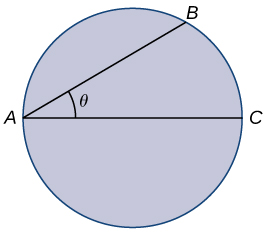
\includegraphics[width=0.5\textwidth]{pool.jpeg}
	\end{center}
\end{figure}
\begin{enumerate}
	\item Find a function that measures the total amount of time it takes to reach the drowning person as a function of the swim angle,  $\theta$.
	      \vspace{7cm}
	\item Find at what angle  $\theta$ the lifeguard should swim to reach the drowning person in the least amount of time.
\end{enumerate}

\end{problem}




\end{document}
